% --------------------------------------------------------------
% This is all preamble stuff that you don't have to worry about.
% Head down to where it says "Start here"
% --------------------------------------------------------------
 
\documentclass[12pt]{article}
 
\usepackage[margin=1in]{geometry} 
\usepackage{amsmath,amsthm,amssymb,scrextend}
\usepackage{fancyhdr}
\usepackage{enumitem}
\usepackage{amsmath}
\usepackage{amssymb}
\usepackage{textcomp}
\usepackage{fancybox}
\usepackage{tikz}
\usepackage{tasks}
\pagestyle{fancy}
\usepackage[makeroom]{cancel}
\usepackage{graphicx}
\usepackage{caption}
\usepackage{mwe}
\usepackage{tikz}
\usetikzlibrary{positioning}

\newcommand{\N}{\mathbb{N}}
\newcommand{\Z}{\mathbb{Z}}
\newcommand{\I}{\mathbb{I}}
\newcommand{\R}{\mathbb{R}}
\newcommand{\Q}{\mathbb{Q}}
\renewcommand{\qed}{\hfill$\blacksquare$}
\let\newproof\proof
\renewenvironment{proof}{\begin{addmargin}[1em]{0em}\begin{newproof}}{\end{newproof}\end{addmargin}\qed}
% \newcommand{\expl}[1]{\text{\hfill[#1]}$}
 
\newenvironment{theorem}[2][Theorem]{\begin{trivlist}
\item[\hskip \labelsep {\bfseries #1}\hskip \labelsep {\bfseries #2.}]}{\end{trivlist}}
\newenvironment{lemma}[2][Lemma]{\begin{trivlist}
\item[\hskip \labelsep {\bfseries #1}\hskip \labelsep {\bfseries #2.}]}{\end{trivlist}}
\newenvironment{problem}[2][Problem]{\begin{trivlist}
\item[\hskip \labelsep {\bfseries #1}\hskip \labelsep {\bfseries #2.}]}{\end{trivlist}}
\newenvironment{exercise}[2][Exercise]{\begin{trivlist}
\item[\hskip \labelsep {\bfseries #1}\hskip \labelsep {\bfseries #2.}]}{\end{trivlist}}
\newenvironment{reflection}[2][Reflection]{\begin{trivlist}
\item[\hskip \labelsep {\bfseries #1}\hskip \labelsep {\bfseries #2.}]}{\end{trivlist}}
\newenvironment{proposition}[2][Proposition]{\begin{trivlist}
\item[\hskip \labelsep {\bfseries #1}\hskip \labelsep {\bfseries #2.}]}{\end{trivlist}}
\newenvironment{corollary}[2][Corollary]{\begin{trivlist}
\item[\hskip \labelsep {\bfseries #1}\hskip \labelsep {\bfseries #2.}]}{\end{trivlist}}
 
\setlength{\parindent}{0pt}
\begin{document}
 \settasks{
	counter-format=(tsk[r]),
	label-width=4ex
}
% --------------------------------------------------------------
%                         Start here
% --------------------------------------------------------------

\lhead{Math 632}
\chead{Renewal Process}
\rhead{Meenmo Kang}

\begin{section}{Renewal Process}
\subsection{Law of Large Number}
$$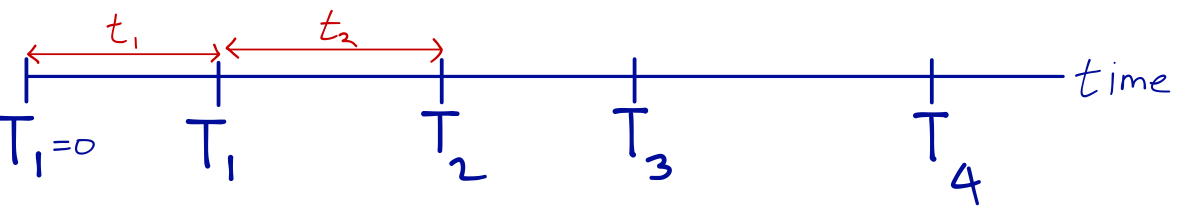
\includegraphics[height=1.4cm, width=9cm]{RP_1.jpeg}$$
\begin{itemize}
    \item Assumption: $\{t_i\}_{i\ge 1}$ are IID non-negative random variables.

    \item Common CDF: $F(t) = P(t_i\le t)$ where $F$ is a distribution with $F(0)= P(t_i\le 0) = 0.$
        \begin{itemize}
            \item At time 0, $t_i$ ends and the following $t_{i+1}$ starts.
            \item i.e. $T_n = t_1+\ldots + t_n$ gives the time $t_n$ ends. (for $n\ge 1)$
        \end{itemize}
        
    \item Common Mean: $\mu = \mu_F = E(t_i)$
    \item $N(t) = \max\{n:T_N\le t\} = $the number of events in [0,t]
    \item Special case: rate $\lambda$ Poisson process whose $\{t_i\}\sim$ IID Exp($\lambda$).
\end{itemize}

\subsubsection{Example}
\begin{enumerate}[label=(\roman*)]
    \item Let $x$ is a recurrent state for a Markov chain. Start the Markov chain at $x$. $T_0 = 0$ and denote $T_n$ as time of $n^{th}$ return to $x$. So $t_i = T_i-T_{i-1}$. Then $\{t_i\}\ge 1$ are IID, so this is a renewal process.
    
    \item Imagine a machine that alternates between a functional state and being under repair. Assume that after repair, the machine is again {\sl like new}.\\
    
    $s_i$ = length of the $i^{th}$ functioning cycle. \qquad\quad
    $u_i = $ length of the $i^{th}$ repair cycle.\\
    $t_i = s_i + u_i$
    $$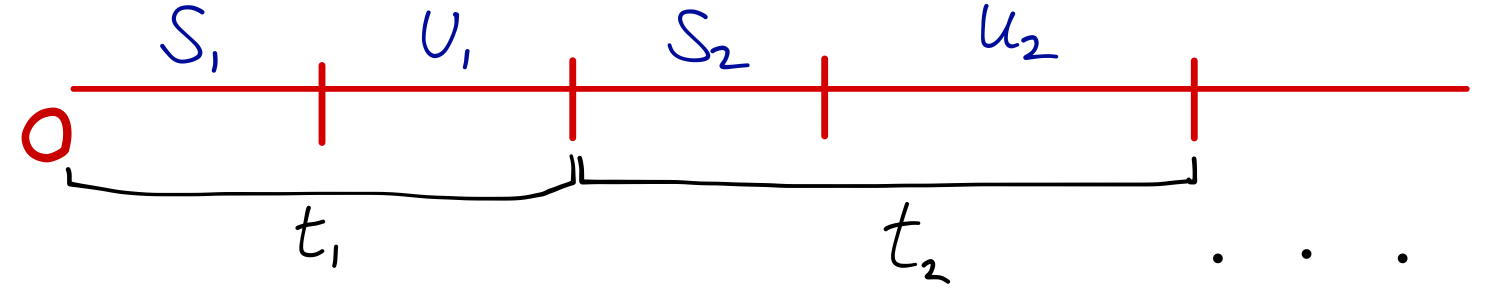
\includegraphics[height=1.4cm, width=9cm]{RP_2.jpeg}$$
    
\end{enumerate}

\vspace{1\baselineskip}
\subsubsection{Theorem 3.1}
Law of Large Number(LLN) for the counting process:
\begin{align}
    \frac{N(t)}{t} \to \frac{1}{\mu}  \tag{ as $t\to \infty$, with probability 1}
\end{align}

{\sl Proof}\\ 
Recall the Strong Law of Large Number(SLLN): if $\{X_i\}$ and IID, 
$$X_i\ge 0,\; S_n = \sum\limits_{i=1}^n x_i$$ then 
$$\frac{S_n}{n}\to EX_1\quad \text{with probability 1}$$

Applying SLLN to $\{t_i\}:$
$$\frac{T_n}{n} \xrightarrow[n\to\infty]{w.p.1} \mu$$

Let $t\to\infty$.
$$\underbrace{\frac{T_{N(t)}}{N(t)}}_{\mu} \le
\underbrace{\frac{t}{N(t)}}_{\mu\text{ as }t\to\infty}\le
\underbrace{\frac{T_{N(t)+1}}{N(t)+1}}_{\substack{{\mu}\\ \text{This works}\\ \text{even in the case} \\ {$\mu=\infty$ }}} \cdot 
\underbrace{\frac{N(t)+1}{N(t)}}_1$$
$$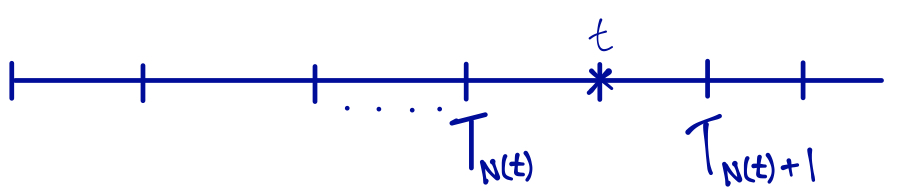
\includegraphics[height=1.4cm, width=9cm]{RP_3.jpeg}$$
\captionof*{}{as $t\to\infty,\;N(t)\to\infty$}


\vspace{2\baselineskip}
\subsubsection{Renewal-reward Process}
To the $i^{th}$ cycle is associated a random {\sl renewed} $r_i$.\\

Assumption: $$\{(t_i,r_i)\}_{i\ge 1}=\{(t_i,r_i),(t_2,r_2),...\}$$ are IID.


$$R(t) = \sum\limits_{i=1}^{N(t)} r_i = \text{total} \textit{ renewal }  \text{up to time $t$}$$

\subsubsection{Theorem 3.3}
Assume $E(r_i)$ is finite. Then
$$\frac{R(t)}{t} \xrightarrow[t\to\infty]{w.p.1} \frac{E(r_1)}{E(t_1)}$$

Check if there's something more

\subsubsection{Example} 
Machine with cycles of functioning $(s_1,s_2,s_3,...)$ and repair $(u_1,u_2,u_3,...)$ Over the long term, what fraction of time is the machine functional?

\vspace{2\baselineskip}
Let $t_i = s_i + u_i$ (cycle length) and $r_i = s_i$ ("reward" = length of functional cycle).
$$\frac{R(t)}{t} = \frac{1}{t} \sum\limits_{i=1}^{N(t)} s_i
=\frac{\text{functional time up to time $t$}}{t}+\underbrace{\frac{\text{small discrepancy}}{t}}_0$$

$$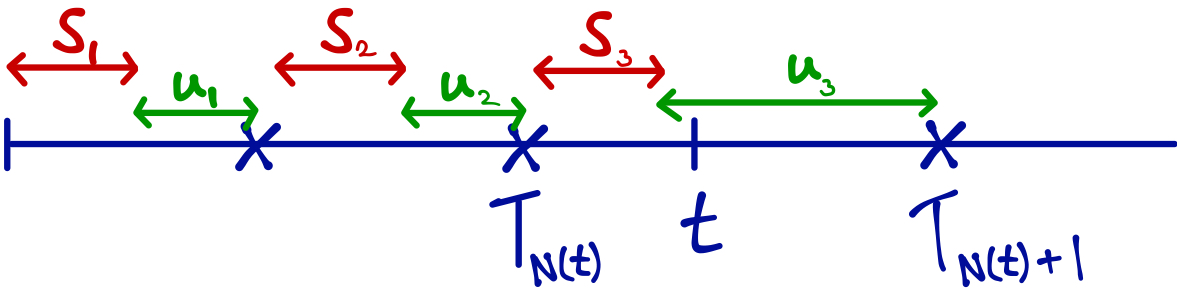
\includegraphics[height=1.5cm, width=10cm]{RP_4.jpeg}$$


\vspace{1\baselineskip}
\subsubsection{Example: Car replacement policy}
Let A be the price at a car after the trade-in. She keeps the car until either the car breaks down or car is $T$ years old. Let $h(t)=$PDF of the lifetime of this car. If the car breaks down, there is an additional cost $B$ when the car is traded in. What is the long-term cost per time unit at this policy?\\

Assumption: $$\frac{E(r_1)}{E(t_1)}$$

Recall: If Y has PDF $h$ then 
$$E[g(Y)]=\int_0^\infty yh(y)dy$$

\begin{align}
    E(t_i) = \int_0^T yh(y)dy + T\int_T^\infty h(y)dy \tag{since T is maximum time for a period} \nonumber
\end{align}
$$E[r_i] = A+B\underbrace{\int_0^T h(y)dy}_{
\substack{
\text{probability that}\\ \text{can break down} \\ \text{before time T}}}$$

\newpage
\subsection{Age and Residual Lifetime} 
$$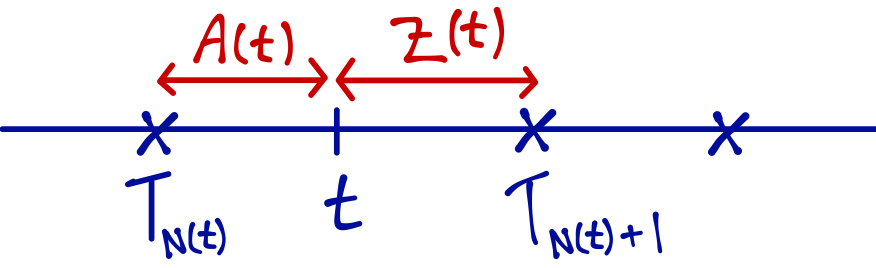
\includegraphics[height=1.7cm, width=10cm]{RP_5.jpeg}$$
$$A(t) = \text{age at the current cycle} = t - T_{N(T)}\qquad
Z(t) = \text{residual lifetime} = T_{N(t)+1} - t$$
\hfill (also called forward recurrent time)

\subsubsection{Example} 
Consider a Poisson process with rate $\lambda$. For every $t$, what are the distribution's of $A(t)$, $Z(t)$, and $Z(t)\sim \exp(t)$?
$$P(A(t)> u) = P(\underbrace{N(t-u,t] = 0}_{\text{Poisson}})=e^{-\lambda t}$$
Except for the cut-off due to the time origin, $A(t)$ is also exponential.

Claim: Let $t_1' = Z(t) = T_{N(t)+1} -t \quad t_i' = t_{N(t)+i},\; i\ge 2$\\
Then $\{t_i'\}_{i\ge 1}$ are independent and $\{t_i'\}_{i\ge 2}$ are IID, with the same distribution F.

\subsubsection{Definition} Let  $S$ be an $\mathbb{Z}_{\ge 0}$ valued random variable. Then $S$ is a \underline{stopping time} for the sequence $\{t_i\}_{i\ge 1}$ if $\{S=n\}$ depends only on $t_1, ..., t_n$.

\subsubsection{Lemma} Let $\{t_i\}_{i\ge 1}$ be IID and $S$ a stopping time. Then $\{t_{s+i}\}_{i\ge 1}$ is independent of $(S, \{t_i\}_{i\le s})$ and $\{t_{s+i}\}_{i\ge 1} \overset{d}{=} \{t_i\}_{i\ge 1}$

\vspace{2\baselineskip}
{\sl Proof}\\
$$P\{\underbrace{S=n,\; (t_1,...,t_n)\in B,}_{\text{An event determined by $(t_1,...,t_n)$}} (t_{n+1},t_{n+2},...)\in U\}$$
$$=P\{S=n,\;(t_1,...,t_n)\in B\}\cdot \underbrace{P\{(t_{n+1},t_{n+2}...)\in U\}}_{P\{(t_1,t_2,...)\in U\}}$$

\newpage
Analogy from recurrent, aperiodic with invariant $\pi$:
$$P_x(X_n=y)\xrightarrow{n\to\infty} \pi(y)$$

Guided by the Markov chain example, we look for a limit distribution for $(A(t), Z(t)).$ The ideal result would be 
$$P(A(t)>x,\;Z(t)>y)\xrightarrow{t\to\infty} \text{ (something) }$$
We don't have the technology for proving this. But we can establish a slightly weaken result.
$$\frac{1}{t}\int_0^t P(A(s)>x,\;Z(s)>y)ds \xrightarrow{t\to\infty}\text{ (something) }$$
\begin{align}
    \frac{1}{t}\int_0^t P(A(s)>x,\;Z(s)>y)ds & = \frac{1}{t}\int_0^t E[\underbrace{1_{A(s)>x,\;Z(s)>y}}_{\substack{\text{indicator r.v.} \\ \text{of the event} \\ \text{$\{A(s)>x,Z(s)>y\}$}}}ds] \nonumber \\
    &=E[\underbrace{\frac{1}{t}\int_0^t 1_{A(s)>x,\;Z(s)>y}ds}_{\substack{
    \text{This average inside the E[..] } \\ \text{we can handle with the} \\ \text{renewal-reward LLN}    }}] \nonumber
\end{align}

\subsubsection{Theorem 3.9}
$$\lim\limits_{t\to\infty}\frac{1}{t}\int_0^t1_{A(s)>x,\;Z(s)>y}ds
=\frac{1}{E(t_1)}\int_{x+y}^\infty P(t_1>z)dz \text{ w.p.1, for any $x,y\ge 0$}$$

$$\frac{1}{t}\int_0^t1_{A(s)>x,Z(s)>y}ds = \frac{1}{t}\sum\limits_{i=1}^{N(t)}\int_{T_{i-1}}^{T_i} 1_{A(s)>x,\;Z(s)>y}ds+ \underbrace{\frac{1}{t}}_{\substack{0 \\ \text{as $t\to\infty$}}}\int_{T_{N(t)}}^t 1_{A(s)>x,\;Z(s)>y}\; ds \;\le\; t_{N(t)+1}$$
$$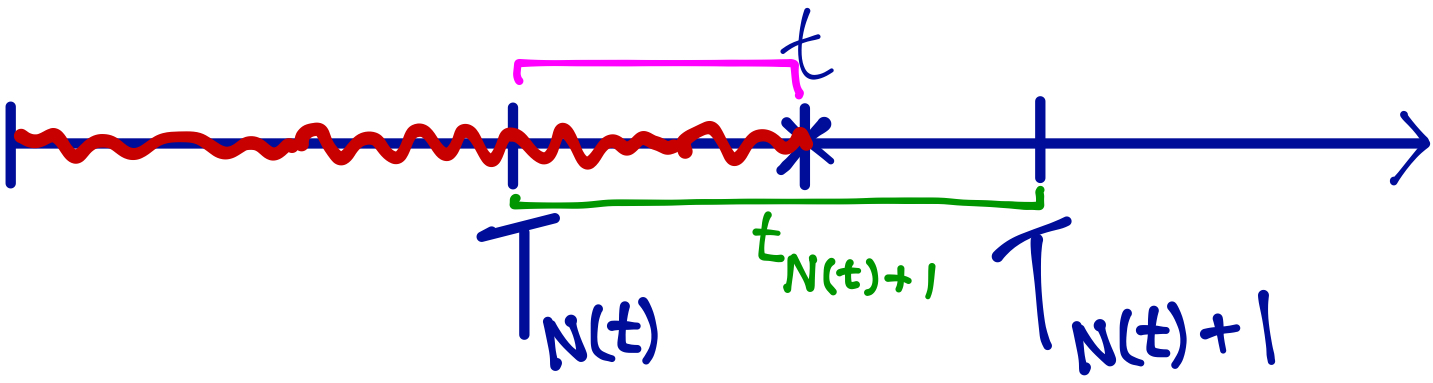
\includegraphics[height=1.4cm, width=9cm]{RP_6.jpeg}$$
Let's calculate $r_i =$
$$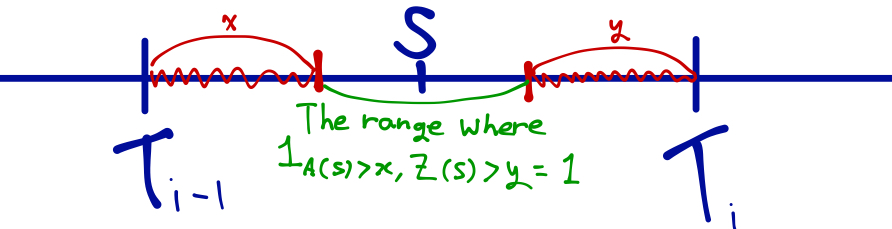
\includegraphics[height=1.7cm, width=9cm]{RP_7.jpeg}$$
\underline{2 cases}:
$$\begin{cases}
x+y\le t_i: r_i = t_i - (x+y)\\
x+y>t: r_i = 0
\end{cases}$$

Notation: for red $x,\; x^+ = \max(x,0)$. e.g. 7^+ = 7, (-3)^+ = 0\\

r_i = (t_i-(x+y))^+.\\

By the renewal-reward LLN,
$$\lim\limits_{t\to\infty}\frac{1}{t}\sum\limits_{i=1}^{N(t)} r_i = \frac{E(r_1)}{E(t_1)}$$

Useful formula: For $X\ge 0,$ then 
$$E(X) = \int_0^\infty P(X>s)ds.$$
{\sl proof.}
\begin{align}
    E(X) &= E\left(\int_0^X ds\right) = E\left(\int_0^\infty 1_{X>s}ds\right) \nonumber \\
    &=\int_0^\infty E(1_{X>s})ds = \int_0^\infty P(X>s)ds \nonumber \\
    E(r_1) & = E\left[(t_1-(x+y))^+\right] = \int_0^\infty P\{\underbrace{(t_1-(x+y))^+>s}_{\text{for }s>0}\}ds \nonumber \\ 
    \tag*{$(t_1-(x+y))^+>s \Leftrightarrow t_1-(x+y)>s$} \\
    \tag*{$\Leftrightarrow t_1 > s+x+y$} \\
    &=\int_0^\infty p(t_1 >s+x+y) ds = \int_{x+y}^\infty P(t_1>z) \nonumber
\end{align}

{\sl Fact}: if random variables $X_n\to X$ w.p.1 and $|X_n|\le c$ (constant) $\forall n$ then $E(X_n)\to E(X)$\\

Take E[...] over Theorem 3.9:
$$\lim\limits_{t\to\infty}\frac{1}{t}\int_0^tP(A(s)>x,\;Z(s)>y)ds = \frac{1}{E(t_1)}\int_{x+y}^\infty P(t_1>z)dz$$

Let $A(\infty),\;Z(\infty)$ represent {\sl limiting} or long-term age and residual lifetime. Our result gives
$$P(A(\infty)>x,\;Z(\infty)>y) = \frac{1}{E(t_1)}\int_{x+y}^\infty P(t_1>z)dz$$

$$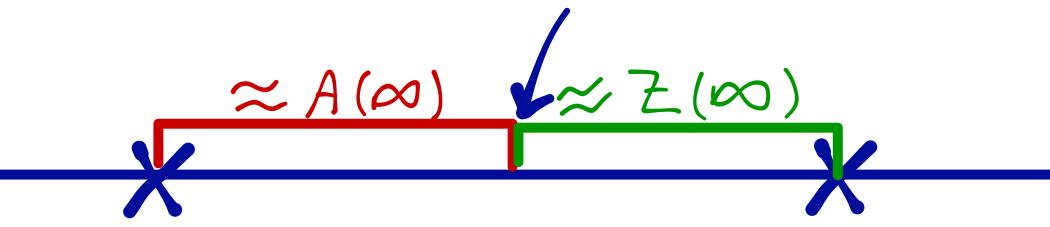
\includegraphics[height=1.4cm, width=9cm]{RP_8.jpeg}$$
\subsubsection{Example: $t_i\sim$ Exp($\lambda),\; E(t_1) = \frac{1}{\lambda}$}

\begin{align}
    P(A(\infty)>x,\;Z(\infty)>y) &= \frac{1}{E(t_1)}\int_{x+y}^\infty P(t_1>z)dz \nonumber \\
    &=\lambda \int_{x+y}^\infty e^{- \lambda z}dz = e^{-\lambda x}\cdot e^{-\lambda y} \nonumber \\
    &\Rightarrow \text{so $A(\infty)$ and $Z(\infty)$ are independent and both are Exp($\lambda$)} \nonumber
\end{align}

\subsubsection{Example: $t_i\sim$ Unif(0,1), $Et_1 = \frac{1}{2}$}
\begin{align}
    P(A(\infty)>x,\;Z(\infty)>y) & = \frac{1}{E(t_1)}\int_{x+y}^\infty \underbrace{P(t_1>z)}_{=\begin{cases}1-z & 0<z<1 \\ 0&z\ge 1 \end{cases}}dz \nonumber \\
    &=2\int_{x+y}^1(1-z)dz = 2\int_0^{1-(x+y)}u du = (1-x-y)^2 \nonumber
\end{align}
$$P(A(\infty)>x),\;Z(\infty)>y)=\begin{cases}
0&x+y\ge 1\\ (1-x-y)^2 & x+y <1
\end{cases}$$

Marginals:
\begin{align}
    P(Z(\infty)>y) & = P(A(\infty)>0,\;Z(\infty)>y) = (1-y)^2 \nonumber \\
    P(A(\infty)>x)&= (1-x)^2 \nonumber
\end{align}
$(1-x)^2(1-y)^2 = (1-x-y)^2$ is not true except for some special x,y. Hence $A(\infty)$ and $Z(\infty)$ are not independent.

\vspace{2\baselineskip}
Back to the general results:
$$P(A(\infty>x,\;Z(\infty)>y) = \frac{1}{E(t_1)}\int_{x+y}^\infty P(t_1>z)dz$$
Let's find $g$= PDF of $Z(\infty)$, and also $E(Z(\infty)).$ Assume that $t_1$ has PDF $f_{t_1}$.

$$P(Z(\infty)>y) = P(A(\infty)>0,\;Z(\infty)>y) = \frac{1}{E(t_1)}\int_y^\infty P(t_1>z)dz$$
$$g(y) = -\frac{d}{dy}P(z(\infty)>y) = \frac{P(t_1>y)}{E(t_1)}$$

\subsubsection{Example: $t_1\sim$ Exp$(\lambda)$}
Another useful formula: Assume $X\ge 0,\; h(0)=0$
\begin{align}
    E[h(X)] &= E\left[\int_0^X h'(s)ds\right] = E\left[\int_0^\infty h'(s) 1_{X>s}ds \right]\nonumber \\
    &=\int_0^\infty h'(s)E[1_{X>s}]ds = \int_0^\infty h'(s)P(X>s) ds \nonumber
\end{align}

\vspace{1\baselineskip}
$$g(y) = \frac{P(t_1>y)}{E(t_1)} = \frac{e^{-\lambda y}}{1/\lambda} = \lambda e^{-\lambda y}$$

$$E[Z(\infty)] =\int_0^\infty y g(y)dy = \frac{1}{E(t_1)}\int_0^\infty y P(t_1>y)dy =\frac{\frac{1}{2}E[t_1^2]}{E(t_1)}$$


\subsubsection{Theorem}
Let now $t_1'$ have the distribution of $Z(\infty)$, and $t_2',t_3',...$ have the IID distribution of $t_1$. Then we get a {\sl stationary renewal process} whose probability are constant in time: in particular, P(the number of arrivals in (a,b] = m) = P(the number of arrivals in (s+a,s+b)=m) 

$$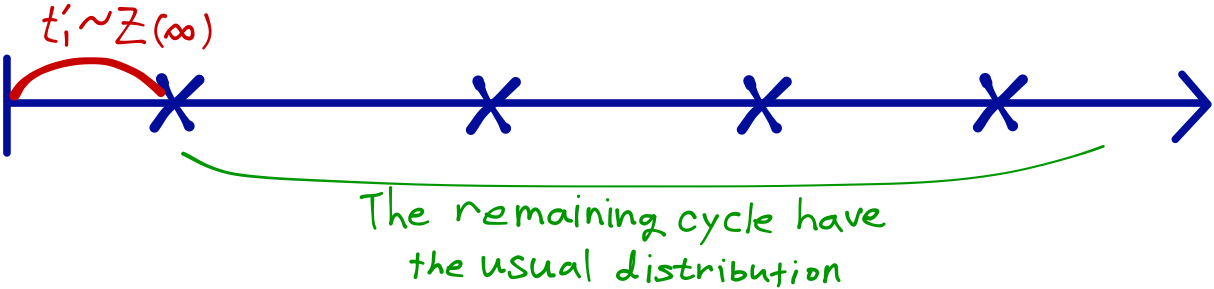
\includegraphics[height=1.9cm, width=9cm]{RP_9.jpeg}$$

\newpage
\subsubsection{Exercise}
Customer come out of the terminal at Poisson rate $\lambda(=10/hr)$. After 7 people have arrived, the shuttle takes off for the 36 min($\frac{6}{10}hr)$ round trip to Hilton. Customers who arrived while the shuttle was gone go elsewhere.



\end{section}
\end{document}